\chapter{Parallele Programmierung}
\lhead{Parallele Programmierung}
High Performance Computing Probleme erfordern spezielle Algorithmen, die
wiederum auf Unterst"utzung durch die Programmiersprachen in Form von
Bibliotheken oder speziellen Sprachkonstrukten angewiesen sind.
In diesem Kapitel wird eine Reihe von solchen Rechenmitteln vorgestellt.

Ziel dieses Kapitels ist nicht, alle behandelten Techniken im Detail
darzustellen, dazu gibt es bessere Quellen auf dem Internet oder in
Form von B"uchern.
Diese Quellen erkl"aren die APIs im Detail, beschreiben, wie man Programme
kompiliert und wie man sie startet. Sie gehen jedoch davon aus, dass der
Entwickler sich bereits dar"uber klar geworden ist, welches Framework
f"ur das vorliegende Problem am besten geeignet ist.
Welche Kriterien anzuwenden sind, um zu dieser Entscheidung zu gelangen,
ist jedoch normalerweise nicht Inhalt der Dokumentation.

Alle Frameworks stellen eine Vielzahl von M"oglichkeiten zur
Verf"ugung, oft mehr als man "uberblicken kann, wenn man sich f"ur
eines entscheiden muss.
Auf welche Features muss man speziell achten? Um diese Auswahl
zu vereinfachen, soll ein typisches Problem in allen zu diskutierenden
APIs gel"ost werden. Dabei zeigen sich St"arken und Schw"achen  in
exemplarischer Weise.

\section{Fallstudie}
\rhead{Fallstudie}
Als Fallbeispiel soll der Gauss-Algorithmus zur Berechnung der Inversen
einer $n\times n$-Matrix verwendet werden. Dabei ist das Ziel weniger,
den letzten Rest Performance herauszuholen, sondern vielmehr zu
illustrieren, welche Art von Konstrukten in einem API zur Verf"ugung
gestellt werden muss, damit die parallele Implementierung effizient
von Statten gehen kann.

\subsection{Der Gauss-Algorithmus}
Wir erinnern an den grundlegenden Gauss-Algorithmus.
Gegeben ist eine regul"are
$n\times n$-Matrix $A$, gesucht wird ihre Inverse $A^{-1}$.
Der Gauss-Algorithmus formt ein Tableau der Form
\begin{equation}
\begin{tabular}{|>{$}c<{$}>{$}c<{$}>{$}c<{$}>{$}c<{$}|>{$}c<{$}>{$}c<{$}>{$}c<{$}>{$}c<{$}|}
\hline
a_{11}&a_{12}&\dots &a_{1n}&1     &0     &\dots &0\\
a_{21}&a_{22}&\dots &a_{2n}&0     &1     &\dots &0\\
\vdots&\vdots&\ddots&\vdots&\vdots&\vdots&\ddots&\vdots\\
a_{n1}&a_{n2}&\dots &a_{nn}&0     &0     &\dots &1\\
\hline
\end{tabular}
\label{starttableau}
\end{equation}
Mit Hilfe von Zeilenoperationen in ein Tableau der Form
\begin{equation}
\begin{tabular}{|>{$}c<{$}>{$}c<{$}>{$}c<{$}>{$}c<{$}|>{$}c<{$}>{$}c<{$}>{$}c<{$}>{$}c<{$}|}
\hline
1     &0     &\dots &0     & c_{11}&c_{12}&\dots &c_{1n}\\
0     &1     &\dots &0     & c_{21}&c_{22}&\dots &c_{2n}\\
\vdots&\vdots&\ddots&\vdots& \vdots&\vdots&\ddots&\vdots\\
0     &0     &\dots &1     & c_{n1}&c_{n2}&\dots &c_{nn}\\
\hline
\end{tabular}
\label{targettableau}
\end{equation}
Die Matrix $C$ ist die gesuchte Inverse: $C=A^{-1}$.

Die Zeilenoperationen beginnen damit, dass ein Pivot-Element ausgew"ahlt
werden muss.
Die Wahl des Pivot-Elements kann die Genauigkeit des Resultates beeinflussen,
entsprechend sind ausgekl"ugelte Strategien entwickelt worden, wie die
Pivot-Elemente am Besten ausgew"ahlt werden sollen. Da dieser Aspekt in
diesem Kapitel nicht wesentlich ist, verwenden wir als Pivot-Elemente die
Diagonalelemente der Matrix. Es werden also der Reihe nach Zeilen-Operationen
mit den Pivot-Elementen $a_{11}$, $a_{22}$ ,$\dots$ ,$a_{nn}$ 
durchgef"uhrt.

Die Pivot-Zeile wird zun"achst durch das
Pivot-Element geteilt wird. Die Matrix-Elemente der Zeile $i$ werden
also nach der Regel
\begin{equation}
a_{ij}'=\frac{a_{ij}}{a_{ii}}
\label{red}
\end{equation}
ersetzt.
An der Stelle des Pivot-Elements steht jetzt eine 1.

In Zeile $k$ steht in der Pivot-Spalte $a_{ki}$. Dieses Element kann
zu $0$ gemacht werden, indem das $a_{ki}$-fache der Pivot-Zeile
subtrahiert wird. Die Elemente der Zeile $k$ werden also nach
der Regel
\begin{equation}
a_{kj}' = a_{kj} - a_{ki}a_{ij}' 
=a_{kj} - a_{ki}\frac{a_{ij}}{a_{ii}}.
\label{blue}
\end{equation}
Damit werden alle Elemente unter dem Pivot-Elemente zu 0 gemacht.

Durch Wiederholung der Operationen (\ref{red}) und (\ref{blue}) f"ur
alle Pivot-Elemente erreicht man die Tableau-Form
\[
\begin{tabular}{|>{$}c<{$}>{$}c<{$}>{$}c<{$}>{$}c<{$}|>{$}c<{$}>{$}c<{$}>{$}c<{$}>{$}c<{$}|}
\hline
1     &*     &\dots &*     & c_{11}&0     &\dots &0     \\
0     &1     &\dots &*     & c_{21}&c_{22}&\dots &0     \\
\vdots&\vdots&\ddots&\vdots& \vdots&\vdots&\ddots&\vdots\\
0     &0     &\dots &1     & c_{n1}&c_{n2}&\dots &c_{nn}\\
\hline
\end{tabular}
\]
Die linke untere H"alfte des Tableau hat jetzt bereits die gem"asst
(\ref{targettableau}) angestrebte Form.
Man nennt den bisher durchgef"uhrten Teil die Vorw"arts-Reduktion.

Um die rechte obere H"alfte auch noch zu 0 zu machen,
m"ussen weitere Zeilenoperationen angewendet werden. Man nennt diese
Phase des Algorithmus das R"uckw"artseinsetzen.
Da die Diagonal-Elemente immer noch Wert 1 haben, kann dies in Spalte
$i$ mit den Ersetzungen
\begin{equation}
a_{kj}'' = a_{kj}' - a_{ki}'a_{ij}'
\label{green}
\end{equation}
geschehen.

Wir sch"atzen den Rechenaufwand f"ur die Durchf"uhrung des Algorithmus ab.
Die Division durch das Pivot-Element (\ref{red}) ben"otigt $2n$ Operationen.
Damit werden in den $n-i$ Zeilen unter dem Pivot-Element jeweils
$2n\cdot 2=4n$ Operationen durchgef"uhrt.
F"ur das R"uckw"artseinsetzen sind nochmals jeweils $(i-1)\cdot 4n$ Operationen
notwendig. Insgesamt braucht der Algorithmus also
\[
2n^2
+
\sum_{i=1}^n4n(n-i)+\sum_{i=1}^n 4n(i-1)
=2n^2+4n(n-1)\sum_{i=1}^n1=2n^2+4n(n-1)n=4n^3-2n^2
\]
Operationen.

Nat"urlich hat der Algorithmus in dieser Form noch einiges
Optimierungspotential. So ist es zum Beispiel nicht n"otig, jeweils
die ganze Zeile zu berechnen, es reicht, diejenigen Teile zu
berechnen, die in sp"ateren Schritten ben"otigt werden. 

\subsection{Implementation}
Die Implementation des Algorithmus in C ist unproblematisch. Der Quellcode
kann im zu diesem Skript geh"orenden Repository auf Github gefunden
werden. 

Der Inhalt des Tableau (\ref{starttableau}) wird in einem Array {\tt a}
abgelegt. Das Makro {\tt M} mit der Defintion
\verbatiminput{M.c}
vereinfacht den Zugriff auf den Array {\tt a}. Damit l"asst sich die 
Vorw"artsredunktion wie folgt formulieren:
\verbatiminput{sequentialforward.c}
Das R"uckw"artseinsetzen ist noch einfacher, weil die Pivot-Zeile
nicht erst dividiert werden muss.
\verbatiminput{sequentialbackward.c}
Die Laufzeit des Algorithmus (Abbildung~\ref{laufzeit-sequentiell})
zeigt die erwartete $O(n^3)$ Abh"angigkeit. Lineare Regression f"ur 
die Messpunkte liefert den Exponenten $2.985$, als sehr nahe am
theoretischen Exponenten 3.
\begin{figure}
\begin{center}
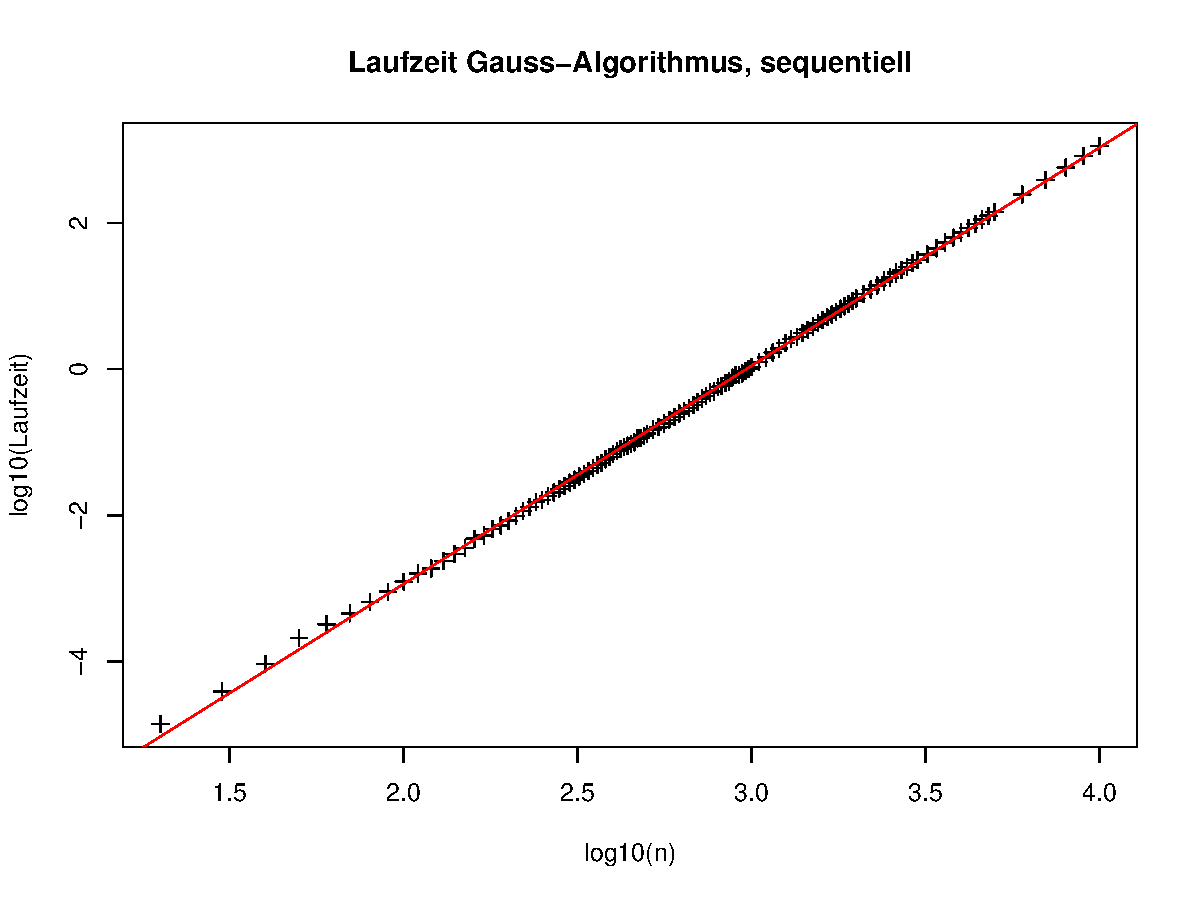
\includegraphics[width=\hsize]{images/gauss-seq.pdf}
\end{center}
\caption{Laufzeit des Gauss-Algorithmus, sequentielle Implementation
\label{laufzeit-sequentiell}}
\end{figure}

\subsection{Parallelisierung}
Die Zeilenoperationen des Gaussalgorithmus k"onnen mit folgenden
Einschr"ankungen parallelisiert werden:
\begin{enumerate}
\item Mit den Zeilenoperationen darf erst dann begonnen werden,
wenn die Pivot-Zeile dividiert worden ist. Genauer: die Elemente
in der Spalte $j$ k"onnen erst berechnet werden, wenn das Element in Spalte
$j$ in der Pivot-Zeile berechnet worden ist.
\item Bei der Bearbeitung von Zeile $k$ darf das Matrixelement $a_{ki}$
erst dann ver"andert werden, wenn es nicht mehr f"ur die Durchf"uhrung
der Zeilenoperation ben"otigt wird. Dies kann auf verschiedene Arten
geschehen.
Das Element $a_{ki}$, mit dem alle Elemente
der Pivot-Zeile multipliziert werden, bevor sie von der Zeile $k$ subtrahiert
werden, wird nach dieser Zeilen-Operation gar nicht mehr ben"otigt.
Die ganze Spalte $i$ wird nach der Zeilen-Operation nicht mehr ben"otig,
daher m"ussen die Operationen (\ref{blue}) auf die Spalte gar nicht
angewendet werden. Damit verschiendet auch das Problem.
\end{enumerate}

Jeder Gauss-Schritt hat eine kleinere Menge von Zeilen-Operationen auszuf"uhren,
da ja nur die Zeilen $k>i$ bearbeitet werden m"ussen.
Beim R"uckw"artseinsetzen steht dann erst eine grosse Zahl von
Zeilenoperationen an, deren Zahl laufend kleiner wird.
Wie auch immer
man dies parallelisiert, steht mit zunehmendem Fortschritt immer
weniger Arbeit zur Parallelisierung zur Verf"ugung.

Die Operationen des R"uckw"artseinsetzens werden erst nach vollst"andiger
Vorw"artsreduktion ausgef"uhrt, weil sich damit die kleinstm"ogliche
Anzahl Operationen in einem sequentiellen Programm realisieren l"asst.
In einem parallelisierten Algorithmus kann jedoch mit den Operationen
des R"uckw"artseinsetzens bereits vorher begonnen werden. Zwar werden damit
im linken Teil des Tableau einige "uberfl"ussige Operationen ausgef"uhrt,
diese k"onnen aber parallel zu den Operationen der Vorw"artsreduktion
ausgef"uhrt werden.
Da das R"uckw"arts\-einsetzen entf"allt, entsteht ein einfacherer Algorithmus,
mit vergleichbarer Laufzeit:
\verbatiminput{unidirectional.c}
Dieser unidirektionale Algorithmus ist einfacher zu parallelisieren, hat
aber praktisch die gleiche Laufzeit, wie man in Abbildung~\ref{gauss-uni}
sehen kann.
\begin{figure}
\begin{center}
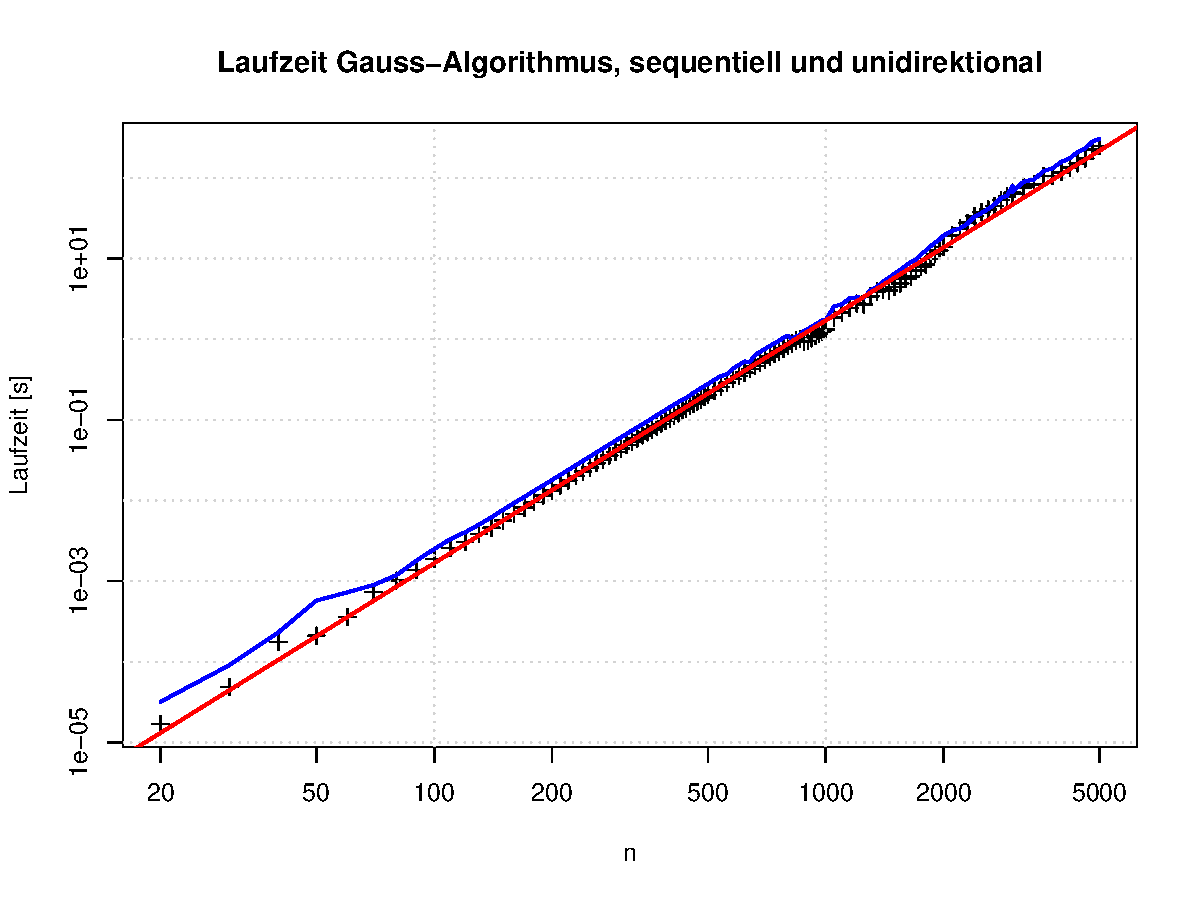
\includegraphics[width=\hsize]{images/gauss-uni.pdf}
\end{center}
\caption{Laufzeit des unidirektionalen Gauss-Algorithmus. Die blaue Kurve
zeigt zum Vergleich die Daten des originalen Algorithmus, f"ur grosse
$n$ ist kein Unterschied feststellbar.
Lineare Regression (rote Gerade) liefert den Exponenten $2.990$.
\label{gauss-uni}}
\end{figure}

\section{Problemkatalog}
Wir stellen hier die Funktionen zusammen, die von einer
Parallelisierungstechnologie bereitgestellt werden m"ussen, um das Problem
der Fallstudie zu l"osen.

\subsection{Thread-Erzeugung}
Parallelisierung verlangt, dass eine angemessene Zahl von Threads erzeugt
werden k"onnen muss.

Wieviele Threads sinnvoll oder optimal sind, l"asst sich oft nicht
direkt aus dem Source-Code ableiten.
Von
Daten-Lokalit"at und Abh"angigkeiten zwischen einzelnen Datenelementen
h"angt ab, in welchem Mass die Arbeit parallelisiert werden kann.
Von Zugriffsmuster und Datenumfang h"angt ab, wie viele Threads
laufen k"onnen, ohne dass sie sich gegenseitig den Cache streitig machen.
Daher muss es m"oglich sein, die Zahl der Threads zu kontrollieren.

\subsection{Scope}
Wann immer ein Code-Segment parallelisiert wird, muss unterschieden
werden k"onnen zwischen Thread-spezifischen Variablen und globalen
Variablen.
Wir betrachten dazu das folgende Codebeispiel, der gleich mehrere Hindernisse
illustriert: 
\begin{verbatim}
int     i, k;
float   s = 0;
float   m = 0;
for (i = 0; i < N; i++) {
        s += a[i];
        if (a[i] > m) {
                m = a[i];
                k = i;
        }
}
\end{verbatim}
Er berechnet die Summe aller Werte im Array {\tt a}, das Maximum und den
Index des gr"ossten Wertes.
Eine Parallelisierung dieser Schleife hat mit folgenden Schwierigkeiten
fertig zu werden:
\begin{itemize}
\item
Teilt man die Summe in einzelne Teile auf, die alle von verschiedenen
Threads berechnet werden, dann braucht jeder Thread seine eigene 
Schleifenvariable.
Bei der Parallelisierung sind also mehrere Kopien Variable {\tt i} zu
erstellen.
\item
Die Summe {\tt s} wird in jedem Schleifendurchgang aktualisiert.
Die Aktualisierung liest den aktuellen Wert von {\tt s}, addiert
den aktuellen Wert aus dem Array {\tt a}, und speichert den neuen Wert
in {\tt s}.
Arbeiten mehrere Threads an dieser Schleife, dann besteht die Gefahr,
dass diese Updates sich "uberlagern, und dass dabei einzelne Upates
von anderen "uberschrieben werden.
Bei der Parallelisierung muss also sichergestellt werden, dass die
Operationen \verb/s += a[i];/ atomar ausgef"uhrt werden.
Die Threads werden m"oglicherweise durch die dazu notwendigen Synchronisierung
blockiert.

Alternativ kann man dies erreichen, indem f"ur jeden Thread eine eigene
Kopie der Variable {\tt s} erzeugt wird, und die in jedem Thread
gefunden summiert.
Der letzte Schritt hat keine Entsprechung im Code, nur durch unser
Verst"andnis dessen, was der Code beabsichtigt, sind wir in der Lage
zu erkennen, wie sich die Behandlung von {\tt s} von der Behandlung
{\tt i} unterscheiden.
\item
Die Variable {\tt k} ist nochmals anders:  Nur einer der Threads kann den
richtigen Wert finden.
Erst durch Vergleich des pro Thread gefundenen Maximums in {\tt m}
kann entschieden werden, welches {\tt k} das Resultat der
parallelisierten Version des Algorithmus sein soll.
Auch daf"ur gibt es keine Information im vorhandenen Code.
\end{itemize}

\subsection{Synchronisation}
Die Threads, die an einer Probleml"osung beteiligt sind, werden alle
vergleichbare Arbeit leisten. 
Im Gauss-Algorithmus k"onnen die einzelnen Threads erst weiterarbeiten,
wenn die Division der Pivot-Zeile abgeschlossen ist, und die Division
der Pivotzeile darf erst erfolgen,
wenn alle Threads mit ihren Zeilenoperationen fertig sind.
Diese beiden Punkte im Code heissen Barrierepunkte.

In vielen Anwendungen, in denen Threads mit v"ollig verschiedenen
Aufgaben eingesetzt werden, dienen Synchronisationsprimitive vor allem
dazu, gemeinsame Datenstrukturen davor zu sch"utzen, dass sie durch
gleichzeitige, unkoordinierte Schreibzugriffe inkonsistent werden.
Daher sind die prim"aren Synchronisationsprimitive in Allzwecksprogrammen
vor allem Mutexes, welche den gleichzeitigen Zugriff auf Datenstrukturen
verhindern. Beispiele:
\begin{itemize}
\item Java kennt das {\tt synchronized} keyword, mit dem verhindert werden
kann, dass mehrere Threads auf das gleiche Objekt zugreifen
oder die gleiche Methode ausf"uhren.
\item Die Boost-Bibliothek stellt eine Klasse {\tt boost::mutex} bereit,
welche Methoden {\tt lock} und {\tt unlock} verwenden.
Drei Viertel der Dokumentation zu den Boost-Synchronisations-Primitiven
befassen sich mit diesen Klassen.
\end{itemize}

Diese Synchronisations-Primitve sind jedoch ungeeignet for das vorliegende
Problem.
Bestenfalls k"onnen Sie die Basis sein f"ur die Implementation einer
Barriere dienen.
Ein f"ur HPC geeignetes Thread-API muss also ein Barriere-Konstrukt
zur Verf"ugung stellen.

\subsection{Input/Output}
Die Daten, auf denen eine umfangreiche Berechnung basieren, und die
Daten, die von derselben produziert werden, m"ussen, von Files gelesen
oder in Files geschrieben werden.
Gleichzeitiger Lese- oder Schreibzugriff von mehreren Threads auf dasselbe
File f"uhrt unweigerlich zu korrupten Daten, wenn keine Massnahmen zur
Synchronisierung der Threads getroffen werden. 

Meistens ist paralleles Lesen oder Schreiben nicht einmal sinnvoll, 
jeder Thread berechnet einen anderen Teil der L"osung, welcher in
einen anderen Teil des Output-Files geschrieben werden muss.
Er braucht dazu Daten, die in einem eigenen Teil der Input-Files
gefunden werden k"onnen.

In vielen F"allen l"ost man das Problem dadurch, dass jeweils ein Thread
oder Prozess die Aufgabe "ubernimmt, alle Input-/Output-Operationen
durchzuf"uhren.
Die Daten m"ussen dann vor der eigentlichen Rechnung an die verschiedenen
Threads oder Prozesse verteilt werden.
Nach Abschluss der Rechnung m"ussen die Resultate von diesem Thread wieder
eingesammelt werden.

Eine bessere L"osung stellen Fileformate zur Verf"ugung, welche paralleles
Schreiben explizit unterst"utzen. {\tt parallel-netcdf} ist ein Projekt,
welches solche Operationen durch verschiedene Prozesse gestattet.

Bei der Parallelisierung f"ur einen Compute-Cluster verliert ausserdem
das Konzept eines Files grunds"atzlich seine Bedeutung.
Die einzelnen Knoten des Clusters haben m"oglicherweise gar kein Filesystem
gemeinsam mit dem Knoten, welcher die Rechnung steuert. 
Die Parallelisierungsmethode muss also File-Operationen reimplementieren,
damit sie f"ur die Cluster-Infrastruktur sinnvoll werden.

\section{Pthreads}
\rhead{Pthreads}
Posix Threads sind das standardisierte API f"ur Thread-Programmierung
und Posix-Systemen.
Das API ist vollst"andig in den Manual-Pages dokumentiert, wir gehen
daher nur auf die Funktionen ein, die f"ur die Beispielimplementation
ben"otigt werden. Im Laufe der Rechnung muss eine Anzahl von Threads
gestartet werden, die am Ende wieder beendet werden m"ussen.

\subsection{Erzeugung von Threads}
Damit alle Threads ordnungsgem"ass beendet werden k"onnen, wird die Information
"uber die Threads in einer Struktur
\begin{verbatim}
typedef struct {
        int        min;
        int        max;
        pthread_t  thread;
} thread_info;
\end{verbatim}
gesammelt. Das {\tt thread}-Member ist ein Handle f"ur einen Thread, die
beiden Werte {\tt min} und {\tt max} geben das Interval von $k$-Indizes
an, f"ur die dieser Thread zust"andig ist.

Da eine grosse Zahl von Threads an der Berechnung beteiligt sein kann,
wird ein ganzer Array von \verb+thread_info+-Strukturen in einer
Struktur
\begin{verbatim}
typedef struct {
        float   *a;     // array
        int     n;      // dimensions
        int     nthreads;
        pthread_barrier_t       barrier1;
        pthread_barrier_t       barrier2;
} common_info;
common_info     common;
\end{verbatim}
gespeichert. Diese Struktur enth"alt auch die zwei Barriers, die
im n"achsten Abschnitt besprochen werden. Das Member {\tt a}
zeigt auf den Array mit dem Tableauinhalt, das Member {\tt n} 
bestimmt die Dimensionen des Tableau.

Zum Starten der Threads dient die Funktion \verb+pthread_create+.
Sie verlangt ein Argument, welches Attribute des neu zu startenden
Thread beinhaltet. In unserem Fall sind keine speziellen Attribute
n"otig, so dass die Threads mit dem Befehl
\begin{verbatim}
pthread_attr_t  attr;
pthread_attr_init(&attr);
pthread_create(&info[i].thread, &attr, thread_main, &info[i]);
\end{verbatim}
Das Symbol \verb+thread_main+ ist die Funktion, die vom Thread
ausgf"uhrt werden soll, das vierte Argument ist das Pointer-Argument,
welches der Funktion "ubergeben wird.
Die Funktion muss also als erstes das Argument auf den Typ \verb+thread_info+
casten:
\begin{verbatim}
void    *thread_main(void *arg) {
        // get info about the thread
        thread_info     *this = (thread_info *)arg;
\end{verbatim}
Nat"urlich darf nur ein Thread die Division des Pivot-Elements durchf"uhren.
Man k"onnte dies als klassisches Locking-Problem betrachten, dies ist
jedoch nicht korrekt. Ein Mutex stellt nur sicher, dass nicht mehr als
ein Thread an diesem Teilproblem arbeitet. Ein sp"at an diesem Punkt
im Code ankommender Thread w"urde die Division nochmals durchf"uhren.
Sie h"atte zwar keine Wirkung, weil das Pivot-Element an diesem Punkt
bereits 1 ist. Eine der Optimierungsm"oglichkeiten des Algorithmus
besteht aber darin, das Pivot-Element gar nicht zu dividieren, was
dann zu einem Fehler bei mehrfacher Ausf"uhrung der Pivot-Division
f"uhren w"urde.

Das Pthreads-API erlaubt aber auch, den Handle des aktuellen Threads
zu erhalten und mit den global verf"ugbaren Thread-Handles zu
vergleichen. Damit kann man sicherstellen, dass nur der erste der
gestarteten Threads die Pivot-Division durchf"uhrt:
\begin{verbatim}
if (pthread_self() == info[0].thread) {
        float   pivot = a[i + 2 * n * i];
        for (int j = i; j < 2 * n; j++) {
                a[j + 2 * n * i] /= pivot;
        }
}
\end{verbatim}

Erst wenn der erste Thread die Zeilendivision durchgef"uhrt hat, darf 
die Zeilenoperation in den anderen Zeilen durchgef"uhrt werden. Dazu
dient der API-Aufruf \verb+pthread_barrier_wait+.
Die Members {\tt min} und {\tt max} geben jetzt an, f"ur welche Zeilen
der Thread die Zeilen-Operationen durchf"uhren muss:
\begin{verbatim}
pthread_barrier_wait(&common.barrier1);
for (int k = this->min; k < this->max; k++) {
        if (k != i) {
                float   b = a[i + 2 * n * k];
                for (int j = i; j < 2 * n; j++) {
                        a[j + 2 * n * k] -= this->b * a[j + 2 * n * i];
                }
        }
}
pthread_barrier_wait(&common.barrier2);
\end{verbatim}
Hier wird eine Zeilen-Operation in allen Zeilen durchgef"uhrt.
Jeder Thread arbeitet mit einem anderen $b$, da aber $b$ ohnehin
eine lokale Variable ist, die auf dem Thread-Stack alloziert wird,
entsteht kein Konflikt.

Das Pthread API stellt auch einen Mechanismus zur Verwaltung von
Thread-spezifischem Speicher zur Verf"ugung. Um solchen Speicher
zu verwenden, muss erst ein \verb+pthread_key_t+ erzeugt werden,
welcher in allen Threads als Handle f"ur den Thread-spezifischen
Speicher dient.
Mit dem Key ist auch ein Destruktor verbunden,
der sicherstellt, dass Thread-spezifischer Speicher bei Thread-Ende 
dealloziert wird. Die Zuweisung von Speicher als Thread-spezifischer
Speicher geschieht mit der Funktion \verb+pthread_setspecific+,
f"ur den Zugriff darauf verwendet man die Funktion \verb+pthread_getspecific+.

\subsection{Barriers}
Der Pthreads-Standard definiert auch ein Barrier-Konstrukt, welches
jedoch nicht in allen Pthread-Implementationen tats"achlich vorhanden ist%
\footnote{Barriers fehlen zum Beispiel in FreeBSD und Mac OS X.
In der Beispiel-Implementation im Repository wird im File
{\tt barrier.h} eine Ersatz-Implementation bereitgestellt, welche nur
auf Mutexes und Conditiona variables basiert.}.

Die Verwendung der Barriers ist oben bereits dargestellt worden, es fehlt
nur noch die Initialisierung:
\begin{verbatim}
// initialize the barriers
pthread_barrier_init(&common.barrier1, NULL, common.nthreads);
pthread_barrier_init(&common.barrier2, NULL, common.nthreads);
\end{verbatim}
Die Initialisierung legt die Anzahl der Threads fest, auf die die Barrier
wartet. Das zweite Argument der \verb+pthread_barrier_init+-Funktion
beinhaltet Attribute, im aktuellen Standard sind jedoch keine Werte
f"ur dieses Argument definiert.

\subsection{Rechenleistung}
\begin{figure}
\begin{center}
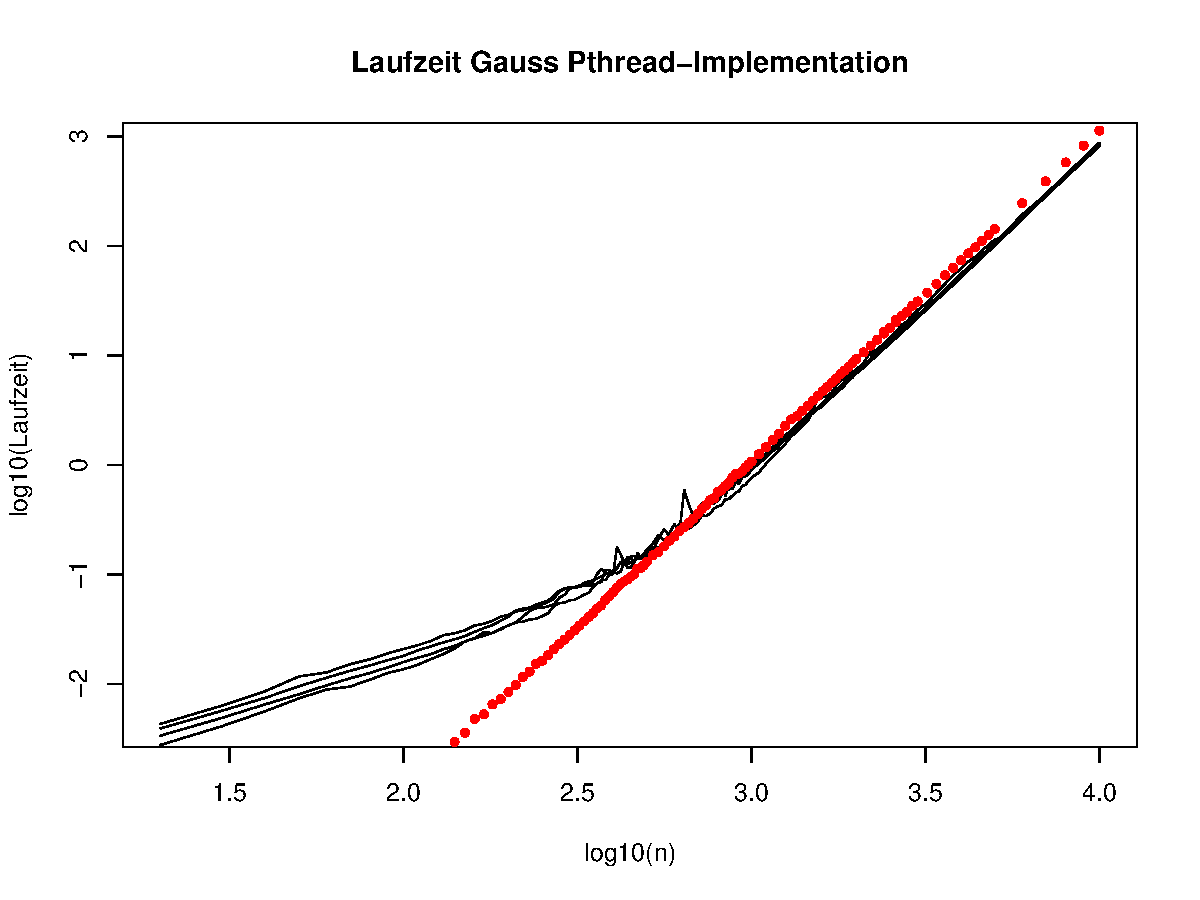
\includegraphics[width=\hsize]{images/gauss-pthread.pdf}
\end{center}
\caption{Laufzeit des mit Pthreads implementierten Gauss-Algorithmus.
Im Vergleich dazu die Laufzeit der sequentiellen Implementierung 
in rot\label{gauss-pthread}}
\end{figure}
Die Messungen in Abbildung \ref{gauss-pthread} zeigen, dass der mit
Pthreads parallelisierte Algorithmus nicht sehr gut skaliert. Dies
d"urfte folgende Ursachen haben:
\begin{itemize}
\item
Die Threads laufen auf verschiedenen CPUs, aber der Speicher wurde
h"ochstwahrscheinlich im ersten Prozess alloziert, die meisten
Speicherzugriffe erfolgen also "uber eine ``fremde'' CPU, und sind
daher langsamer.
\item
Eine grosse Zahl von Threads, die auf den gleichen Speicherbereich
zugreifen, werden den Cache in k"urzester Zeit umw"alzen.
\item
Die einzelnen Threads sind bis auf die Barriers v"ollig unabh"angig.
Die von Ihnen erzeugten Cache-Zugriffe sind daher ungeordnet, jeder
Threads greift ``wild'' durch den ganzen Cache hindurch, so dass
der Performance-Gewinn durch den Cache zusammenbricht.
\end{itemize}
Ausserdem kann man ablesen, dass bei kleinen Problemgr"ossen 
alle Threads zu starten und wieder zu beenden, einen wesentlichen 
Mehraufwand bedeutet, der die Laufzeit eines Algorithmus mit nur
einem Thread deutlich "ubersteigt.

\section{OpenMP\label{openmp-intro}}
\rhead{OpenMP}
Aus den Beobachtungen zur Performance einer Parallelisierung mit
Pthreads kann man ableiten, dass es sinnvoll sein kann,
eine Parallelisierungsmethode zu w"ahlen, bei der die einzelnen
Threads nicht so frei sind.
Parallelisierung muss also mit einer wesentlich feineren Granularit"at
stattfinden, auf der Ebene einzelner Instruktionen oder Kontrollstrukuren.
Genau dies leistet OpenMP \cite{skript:openmp}.

OpenMP ist eine API-Spezifikation f"ur parallele Programmierung.
Die erste Spezifikation f"ur Fortran erschien 1997, die j"ungste 
Version 4.0 wurde im Juli 2013 ver"offentlicht.
Die Spezifikation kann von der OpenMP Website \url{http://www.openmp.org}
heruntergeladen werden.

Gegen"uber Pthreads verlagert OpenMP die Hauptarbeit der Parallelisierung
in den Compiler. 
Im einfachsten Fall gen"ugt es, den Source-Code eines sequentiellen Programs
mit einigen wenigen Pragmas auszuzeichnen, die parallelisierbare
Konstrukte markieren. Der Compiler kann dann daraus parallelen Code
generieren. Insbesondere soll der Programmierer nicht wissen m"ussen, wieviele
Threads an einem parallelen Konstrukt arbeiten, es wird der Implementation
"uberlassen, die optimale Anzahl von Threads zu w"ahlen.

Im Beispiel-Problem ist die Parallelisierung besonders einfach, da
OpenMP Konstrukte f"ur parallel auszuf"uhrende Schleifen bereitstellt.
Durch Hinzuf"ugen eines einzelnen Pragmas entsteht paralleler Code:
\begin{verbatim}
#pragma omp parallel for
for (int k = 0; k < n; k++) {
        if (k != i) {
                float   b = M(a, 2 * n, k, i);
                for (int j = i; j < 2 * n; j++) {
                        M(a, 2 * n, k, j) -= b * M(a, 2 * n, i, j);
                }
        }
}
\end{verbatim}
Das OpenMP Runtime parallelisiert die {\tt for}-Schleife. Dabei wird
angenommen, dass die einzelnen Zeilen voneinander unabh"angig sind, dass
also jeder von OpenMP gestartete Thread eine Zeile bearbeiten kann,
ohne auf Resultate eines anderen Threads warten zu m"ussen.

Auf die Problematik der Variable {\tt b} wurde schon im Pthread-Fall
hingewiesen. Auch hier ist {\tt b} eine lokale Variable, die auf
dem Thread-Stack alloziert wird. W"urde man hingegen $b$ ausserhalb
der Schleife allozieren, w"are nicht mehr klar, dass jeder Thread
eine eigene Kopie der Variable braucht. In diesem Fall m"usste man
mit Hilfe der Direktive {\tt threadprivate} sicherstellen, dass
das OpenMP Runtime jedem Thread eine eigene Kopie der Variable $b$
bereitstellt.

Schaut man sich den Code genauer an, den der Compiler f"ur die Schleife
generiert, stellt sich heraus, dass der Optimizer die Variable $b$
ohnehin entfernt. Sie wird ja in jedem Schleifendurchgang der inneren
Schleife gebraucht, so dass es sich lohnt, den Wert von $b$ in einem
Register zu behalten.

\subsection{Resultate}
\begin{figure}
\begin{center}
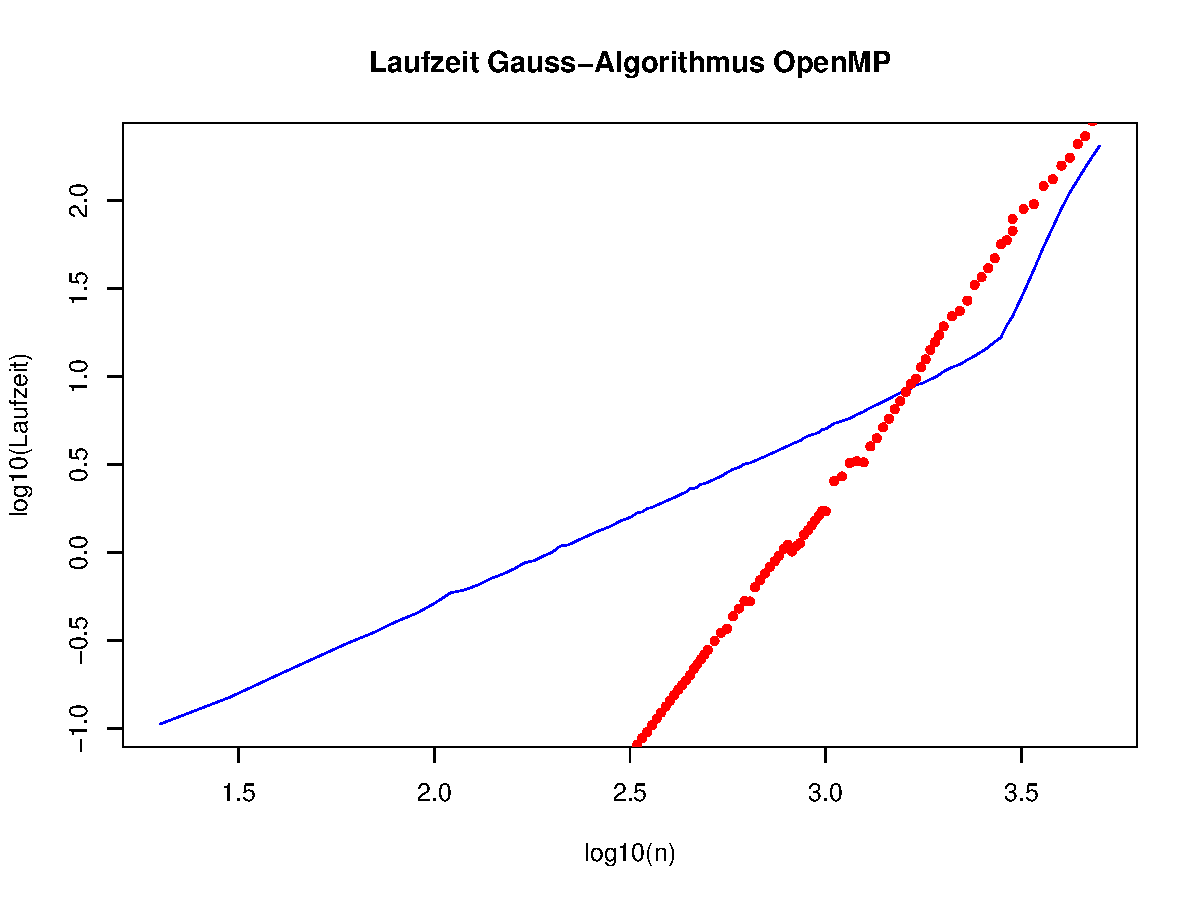
\includegraphics[width=\hsize]{images/gauss-openmp.pdf}
\end{center}
\caption{Laufzeit einer OpenMP-basierten parallelen Implementation
des Gauss-Algorithmus.
Single-Thread Implementation rot, Laufzeit der OpenMP-Implementation
blau\label{openmp-performance}}
\end{figure}
Die Messresultate in Abbildung \ref{openmp-performance}
zeigen, dass die Parallelisierung f"ur kleine $n$
einen grossen Overhead mitbringt, erst ab einer Problemgr"osse von
einigen Tausend ist die OpenMP Implementation der Single Thread
Implementation "uberlegen.

Dann, bei einer Problemgr"osse deutlich ungef"ahr bei der Cache-Gr"osse,
bricht die Performance zusammen, die OpenMP Beschleunigung bringt
keinen Gewinn mehr.

\section{OpenCL\label{opencl-intro}}
\rhead{OpenCL}
Die Open Compute Language \cite{skript:opencl}
erlaubt die plattformunabh"angige Programmierung
f"ur Beschleuniger-Hardware wie zum Beispiel Graphikkarten, wie wir
in Abschnitt \ref{section-beschleuniger} gesehen haben. 
Dort wurde auch bereits das Plattform-Modell besprochen.
F"ur die Art der Parallelisierung ist dieses Modell nur insofern wichtig,
als die Parallelisierung nicht weiter getrieben werden kann als Compute
Units zur Verf"ugung stehen.
Wie allerdings die einzelnen Threads den Compute-Units zugeordnet werden,
wieviele Threads "uberhaupt ausgef"uhrt werden k"onnen, ist der
OpenCL Implementation "uberlassen.
Ja es ist a priori nicht einmal klar, dass der Begriff Thread "uberhaupt
sinnvoll angewendet werden kann.

\subsection{Ausf"uhrungs-Modell von OpenCL}
\subsubsection{Threads}
Ein Thread-Modell orientiert sich an den verf"ugbaren Einheiten, die
parallel arbeiten k"onnen.
Dabei kann das Betriebssystem auch die Illusion von mehr Threads
herstellen, als tats"achlich Verarbeitungseinheiten vorhanden sind.
F"ur einige Beschleunigersystem ist der Begriff eines Threads nicht
sinnvoll, es z"ahlt nur die Berechnung, die durchgef"uhrt worden ist.
Daher verwendet OpenCL ein Ausf"uhrungsmodell, welches sich nicht
an den Ausf"uhrungseinheiten und ihren Threads orientert, sondern an
der gesamten durchzuf"uhrenden Berechnung.

\subsubsection{Work-Items und Kernel}
Eine Berechnungsaufgabe wird in OpenCL in eine Anzahl Work-items
zerlegt.
Eine Kernel ist ein OpenCL Programm, welches f"ur jedes Work-item
ausgef"uhrt wird.
In welcher Reihenfolge die einzelnen work-items abgearbeitet werden,
ist der Implementation "uberlassen.
Ein Work-Item kann beliebig kompliziert sein, in den meisten Beschleunigern
steht jedoch nur sehr wenig Speicher f"ur lokale Variablen zur Verf"ugung.

Die Work-Items bilden ein maximal dreidimensionales Gitter, jedes
{\em work-item} l"asst sich also mittels maximal dreier ganzzahliger 
Indizes identifizieren.
Bei der Konzeption einer L"osung f"ur OpenCL muss sich der
Programmierer also vor allem mit der Frage befassen, wie er die
gesamte Rechnung in {\em work-items} strukturieren kann. 

Work-Items werden in Work-Groups zusammengefasst.
Work-Groups zerlegen das Gitter aller Work-Items in gleich grosse ``Quader''.
Die ``Kantenl"ange'' eines solche Quaders muss also immer ein Teiler
der  ``Kantenl"ange'' des ganzen Gitters sein.

Work-Groups k"onnen nicht beliebig gross sein.
Die Maximale Anzahl Work-Items, die eine Work-Group umfassen kann
wird durch die Implementation festgelegt. 
Mit Hilfe einer Reihe von Abfragefunktionen kann der Programmierer
diese Informationen ermitteln, und die Gruppierung anpassen.

Synchronisation mit Barrieren ist nur innerhalb einer Work-group
m"oglich.
Die Work-group-Gr"osse ist also die maximale Zahl untereinander
synchronisierbarer Work-Items.

Die Indizierung einzelner Work-Items ist sowohl innerhalb einer
Work-Group wie auch global innerhalb aller Work-Items m"oglich.
Wir diskutieren den zweidimensionalen Fall, der eindimensionale und
dreidimensionale Fall ist sinngem"ass. 

Alle Work-Items bilden ein $G_x\times G_y$-Gitter. Die einzelnen
Work-Items werden mit den globalen Indizes $(g_x,g_y)$ adressiert.
Innerhalt einer Workgroup hat ein Work-Item die Koordinaten
$(s_x, s_y)$.
Alle Work-Groups haben die gleichen Dimensionen $S_x\times S_y$.
Die Work-Groups werden ebenfalls "uber ein Koordinatenpaar $(w_x,w_y)$
indiziert. Der Zusammenhang zwischen globalen und lokalen Work-Item
Koordinaten ist daher
\[
(g_x, g_y)=(w_xS_x + s_x, w_yS_y+s_y).
\]
Die Anzahl Work-Groups in jeder Koordinatenrichtung ist $G_x/S_x$
bzw.~$G_y/S_y$.
In Abbildung~\ref{opencl-workitems} ist der Zusammenhang zwischen
Tabelle~\ref{table-work} zeigt die API-Funktionen, mit denen
die Dimensionen sowie die Koordinaten des zur Zeit ausgef"uhrten
Work-Items erfragen kann.

\begin{figure}
\begin{center}
\includegraphics[width=\hsize]{graphics/work-1.pdf}
\end{center}
\caption{Strukturierung der Work-Items
\label{opencl-workitems}}
\end{figure}

\begin{table}
\begin{center}
\begin{tabular}{|>{$}l<{$}|l|}
\hline
\text{Symbol}&Funktion\\
\hline
G_x,\; G_y,\; G_z&\verb+get_global_size(i)+\\
S_x,\; S_y,\; S_z&\verb+get_local_size(i)+\\
g_x,\; g_y,\; g_z&\verb+get_global_id(i)+\\
s_x,\; s_y,\; s_z&\verb+get_local_id(i)+\\
w_x,\; w_y,\; w_z&\verb+get_group_id(i)+\\
G_x/S_x,\;
G_y/S_y,\;
G_z/S_z&\verb+get_num_groups(i)+\\
\hline
\end{tabular}
\end{center}
\caption{API-Funktionen zur Identifikation von Work-Items und Work-Groups.
\label{table-work}}
\end{table}


\subsubsection{Speichermodell}
Work-Groups beinhalten untereinander synchronisierbare Work-Items.
Bei der Abarbeitung dieser Work-Items einer Work-Group werden
lokale Variablen gebraucht,
die die Arbeit in anderen Work-Items nichst st"oren d"urfen.
Solche Variablen beinhalten also Daten, die f"ur jedes Work-Item
privat sind, sie m"ussen mit dem Qualifier \verb+__private+
deklariert werden.

Die Arbeit innerhalb einer Workgroup kann gemeinsame Daten verwenden,
die f"ur andere Work-Groups nicht zug"anglich sein soll.
Solche Variable sind mit dem Qualifier \verb+__local+ zu
deklarieren.

\subsubsection{Command Queues}
Alle Aktionen mit dem OpenCL-Ger"at sind "uber eine sogenannte
Command Queue abzuwickeln. Der typische Ablauf ist also, dass einer
Queue die Input-Daten "ubergeben werden, damit sie ins Ger"at
kopiert werden k"onnen. Dann wird der Queue der auszuf"uhrende
Kernel in Auftrag gegeben, wobei auch die Work-Group-Dimensionen
angegeben werden m"ussen. Nach Abschluss der Rechnung werden die
Resultatdaten mit Hilfe eines Queue-Auftrags zur"uckgelesen.

\subsection{Gauss-Algorithmus}
Die Implementation des Gauss-Algorithmus in OpenCL braucht zun"achst eine
grosse Menge von Code, um das Compute Device zu reservieren.
Die Schnittstelle zum Compute Device ist eine Command Queue,
"uber die Datentransfers zum Speicher des Compute Device und zur"uck
erfolgen.
Auch das Programm f"ur das Compute device wird auf dem
Host kompiliert, und dann dem Compute Device via Command Queue
"ubermittelt.

\subsubsection{Laufzeitumgebung}
In etwas mehr Detail sind folgende Schritte n"otig, um zu einem
Kontext und einer Command Queue mit dem ersten verf"ugbaren
Compute Device zu kommen.
\begin{verbatim}
clGetDeviceIDs(NULL, gpu ? CL_DEVICE_TYPE_GPU : CL_DEVICE_TYPE_CPU,
        1, &device_id, NULL);
cl_context      context = clCreateContext(0, 1, &device_id, NULL, NULL, &err);
cl_command_queue commands = clCreateCommandQueue(context, device_id, 0, &err);
\end{verbatim}
Damit ist jetzt bekannt, f"ur welches Compute Device ein OpenCL-Programm
kompiliert werden muss, was mit folgenden Schritten geschehen kann:
\begin{verbatim}
cl_program      program = clCreateProgramWithSource(context, 1,
                        source, length, err);
\end{verbatim}
Der Pointer \verb+source+ zeigt auf einen Zeichenpuffer, der den Source-Code
des OpenCL Programms enth"alt. Kompilation:
\begin{verbatim}
clBuildProgram(program, 1, &device_id, NULL, NULL, NULL);
\end{verbatim}
Das kompilierte Programm kann jetzt in einen ausf"uhrbaren
Kernel umgewandelt werden, man k"onnte dies mit dem Linken eines
C-Programms vergleichen:
\begin{verbatim}
cl_kernel       kernel = clCreateKernel(program, "invert", &err);
\end{verbatim}

Damit der Kernel ausgef"uhrt werden kann, m"ussen zuerst die Daten
als Memory-Objekte erzeugt und die zugeh"origen Daten an das Compute Device
"ubermittelt werden:
\begin{verbatim}
cl_mem input = clCreateBuffer(context, CL_MEM_READ_ONLY,
        sizeof(float) * n * n, NULL, NULL);
cl_mem output = clCreateBuffer(context, CL_MEM_WRITE_ONLY,
        sizeof(float) * n * n, NULL, NULL);
clEnqueueWriteBuffer(commands, input, CL_TRUE, 0,
        sizeof(float) * n * n, a, 0, NULL, NULL);
clSetKernelArg(kernel, 0, sizeof(cl_mem), &input);
clSetKernelArg(kernel, 1, sizeof(cl_mem), &output);
clSetKernelArg(kernel, 2, sizeof(unsigned int), &n);
\end{verbatim}
Die letzten drei Befehle verbinden den \verb+input+-Puffer mit dem ersten
Kernel-Argument, \verb+output+ wird mit dem zweiten
Argument verbunden, und die in der Variablen \verb+n+ abgelegte
Zahl wird als drittes Argument "ubergeben.

Die bisher verwendeten API-Funktionen sagen "uberhaupt nichts dar"uber
aus, wie die Parallelisierung durchzuf"uhren ist. Dazu ist festzulegen,
wie die einzelnen Work Items strukturiert werden sollen, welche Arbeit
innerhalb eines Work-Items auszuf"uhren ist.
Dabei ist wichtig, dass vor jeder Pivot-Zeilen-Division die Threads
synchronisiert werden m"ussen. Dazu stehen in OpenCL Barriers
zur verf"ugung, diese k"onnen aber nur innerhalb einer Workgroup
synchronisieren. Daher muss dieses Problem von einer einzigen Workgroup
gel"ost werden. Die maximale Gr"osse einer Workgroup kann mit
\begin{verbatim}
clGetKernelWorkGroupInfo(kernel, device_id,
        CL_KERNEL_WORK_GROUP_SIZE, sizeof(local), &local, NULL);
\end{verbatim}
ermittelt werden.
Da diese Gr"osse eher klein ist, typischerweise
zwischen 1 (CPU-Implementation) und einer kleinen Zweierpotenz
(Graphikkarten), bleibt nur eine relativ kleine Zahl von Work Items.
Jedes Work Item muss also mehrere Zeilen der Matrix bearbeiten.
Wie dies genau geschieht, wird bei der Diskussion des Kernel-Codes
besprochen.

Zum Schluss m"ussen die Resultat-Daten gelesen werden, dazu wird wieder
die Command Queue bem"uht:
\begin{verbatim}
clEnqueueReadBuffer(commands, output, CL_TRUE, 0,
        sizeof(float) * n * n, b, 0, NULL, NULL);
\end{verbatim}

Jetzt kann der Kernel ausgef"uhrt werden, wobei auch die Dimensionen
angegeben werden m"ussen. Der Aufruf
\begin{verbatim}
clEnqueueNDRangeKernel(commands, kernel, 1, NULL, &global, &local,
        0, NULL, NULL);
\end{verbatim}
startet den vorher definierten Kernel mit einer indimensionalen
Menge von Work-Items. Die globale Gr"osse ($G_x$) wird im
Argument \verb+global+ "ubergeben, die Work-Group-Gr"osse ($S_x$)
in $\verb+local+$. In unserem Fall sind beide gleich gross.

Der restliche Code im Beispielprogramm dient dazu, die allozierten
Resourcen freizugeben.

\subsubsection{Kernel-Code}
Der Kernel Code im File \verb+gauss.cl+ implementiert den Gauss-Algorithmus.
Der Kernel wird mit drei Argumenten deklariert:
\begin{verbatim}
__kernel void   invert(__global float *input, __global float *output,
        const unsigned int n)
\end{verbatim}
Nach der Diskussion zur Aufteilung der Arbeit in Work-Groups wissen wir,
welcher Bereich von Zeilen von jedem Work-Item bearbeitet werden muss.
Diese Information beh"ort aber zu jedem Work-Item, muss also als 
privat deklariert werden:
\begin{verbatim}
__private unsigned int  min_row;
__private unsigned int  max_row;
\end{verbatim}
Aus der lokalen und globalen Gr"osse kann jetzt die Gr"osse des Blockes
berechnet werden, die ein Work-Item bearbeitet:
\begin{verbatim}
local_size = get_local_size(0);
unsigned int    blocksize = n / local_size;
min_row = get_local_id(0) * blocksize;
max_row = min_row + blocksize;
\end{verbatim}
Der Algorithmus l"auft dann wie gewohnt ab.
Nur Work Item 0 f"uhrt die Pivot-Division durch, und alle anderen
Threads m"ussen darauf warten
\begin{verbatim}
i = 0;
while (i < n) {
    // local id 0 does the pivot operation
    if (get_local_id(0) == 0) {
        float   pivot = 1 / input[i + i * n];
        for (j = 0; j < n; j++) {
            input[j + i * n] = input[j + i * n] * pivot;
            output[j + i * n] = output[j + i * n] * pivot;
        }
    }

    // barrier to wait for the pivot row operation to complete
    barrier(CLK_GLOBAL_MEM_FENCE);

    // now perform the row operations all over the matrix
    for (unsigned int k = min_row; k < max_row; k++) {
        __global float  *outp = output + n * i;
        __global float  *inp = input + n * i;
        if (k != i) {
            j = 0; 
            __global float  *out = output + n * k;
            __global float  *in = input + n * k;
            float   b = in[i];
            // do the remining operations by scalar
            // operations
            while (j < n) {
                out[j] -= b * outp[j];
                in[j] -= b * inp[j];
                j++;
            }
        }
    }

    // don't continue until all threads have completed
    // the row operations
    barrier(CLK_GLOBAL_MEM_FENCE);
    i++;
}
\end{verbatim}

\subsection{SIMD-Operationen}
Die Zeilenoperationen nutzen die F"ahigkeiten einer SIMD-Engine in keiner
Weise aus, und es ist nicht klar, wie der OpenCL-Compiler die innere
{\tt while}-Schleife parallelisieren kann. 
SIMD-Operationen sind vor allem dann gut einsetzbar, wenn die Vektor-Datentypen
von OpenCL verwendet werden.
Zu jedem primitiven Datentyp gibt es in OpenCL Vektordatentypen mit
verschiedenen L"angen,
zum Beispiel gibt es zu {\tt float} die Vektortypen {\tt float2},
{\tt float4}, {\tt float8}  und {\tt float16}.
Verwendet man diese Typen, wird die Anwendung der SIMD-Engine trivial.
Die Grundoperationen sind alle sowohl auf primitive Typen als auch auf
Vektortypen anwendbar, zus"atzlich bietet OpenCL eine grosse Zahl von
Vektor-Funktionen, insbesondere auch Operationen der Vektor-Geometrie.

Im globalen Speicher liegen die Daten jedoch in roher Form vor, als Vektoren
k"onnen Sie erst auf Ebene Compute-Unit verstanden werden.
OpenCL bietet daher Lade- und Speicheroperationen {\tt vload}$n$ und
{\tt vstore}$n$ an , welche den Transfer erm"oglichen.

Mit den Vektor-Operationen l"asst sich die innere Schleife wie folgt
mit Vektoren der L"ange 4 formulieren:
\begin{verbatim}
unsigned int l = 0;
while (j + 4 < n) {
        float4  v = vload4(l, out);
        float4  p = vload4(l, outp);
        v = v - b * p;
        vstore4(v, l, out);

        v = vload4(l, in);
        p = vload4(l, inp);
        v -= b * p;
        vstore4(v, l, in);

        j += 4;
        l++;
}
\end{verbatim}
Die Variable {\tt l} wird dazu verwendet, durch die Vektoren hindurch zu
z"ahlen, {\tt j} z"ahlt die einzelnen Elemente.
Ist die Zeilenl"ange nicht durch vier teilbar, bleiben einzelne 
Elemente zu bearbeiten, was mit der bisherigen skalaren Implementation
erfolgen kann.

\subsection{Resultate}
Die Abbildung \ref{opencl-results} zeigt die Laufzeit der OpenCL-Implementation
des Gauss-Algorithmus. Zun"achst f"allt auf, dass die GPU Implementation
von Nvidia mit Abstand die langsamste ist.
Offenbar kann eine GPU f"ur dieses Problem oder mindestens f"ur die
gew"ahlte Parallelisierung keine Beschleunigung beitragen.
Der Grund daf"ur sind die unvermeidlichen Barriers.
Ohne die Barriers ist die Berechnung um Faktoren schneller, aber nat"urlich
wird dadurch das Resultat falsch.

Die Implementation von AMD und Intel rechnen beide nur mit der CPU%
\footnote{Beide OpenCL Implementation k"onnen nat"urlich auch Graphikkarten
der jeweiligen Hersteller bedienen, nur standen f"ur die Messungen
keine solche zur Verf"ugung. Intel OpenCL kann auch den neueren Intel Phi
Koprozessor unterst"utzen.}.
Es ist daher nicht "uberraschend, dass die erreichte Geschwindigkeit
vergleichbar ist, es "uberrascht aber doch, dass die Performance mit
keiner anderen Parallelisierungstechnologie mithalten kann.
Die Gr"unde daf"ur sind vielf"altig. AMD-OpenCL verwendet nur einen
einzigen Thread f"ur jede Workgroup.
Da der Algorithmus wegen der Synchronisationspunkte nur eine einzige Workgroup
enthalten darf, l"auft er in AMD in nur einem Thread. Die einzige
m"ogliche Beschleunigung kann also daher kommen, dass OpenCL Vektor-Operationen
Verwenden kann und damit die SIMD-F"ahigkeiten der CPUs ausn"utzen kann.
Abbildung~\ref{opencl-simd-amd} zeigt diese Abh"angigkeit.
Offenbar ist AMD OpenCL in der Lage durch die SIMD-Operationen noch eine 
wesentliche Beschleunigung zu erreichen, nat"urlich nicht der maximal
m"ogliche Faktor 4, dazu ist der Overhead des restlichen Algorithmus
zu gross.
Gr"ossere Vektorl"angen bringen keinen Geschwindigkeitsvorteil, die
SIMD-Engine ist nicht genug breit daf"ur.

Etwas entt"auschend ist, dass die SIMD Engine bei der Nvidia-Implementation 
nur gerade einen Faktor 2 herausholen kann (Abbildung~\ref{opencl-simd-nvidia}).
Die Ursache d"urfte hier sein, dass die Daten gr"osstenteils global sind.
Die Parallelisierung wird durch die Hauptspeicherzugriffe gebremst.
Die eigentlichen Rechenoperationen werden dominiert durch die Lade-Operationen
f"ur die Vektoren.

\begin{figure}
\begin{center}
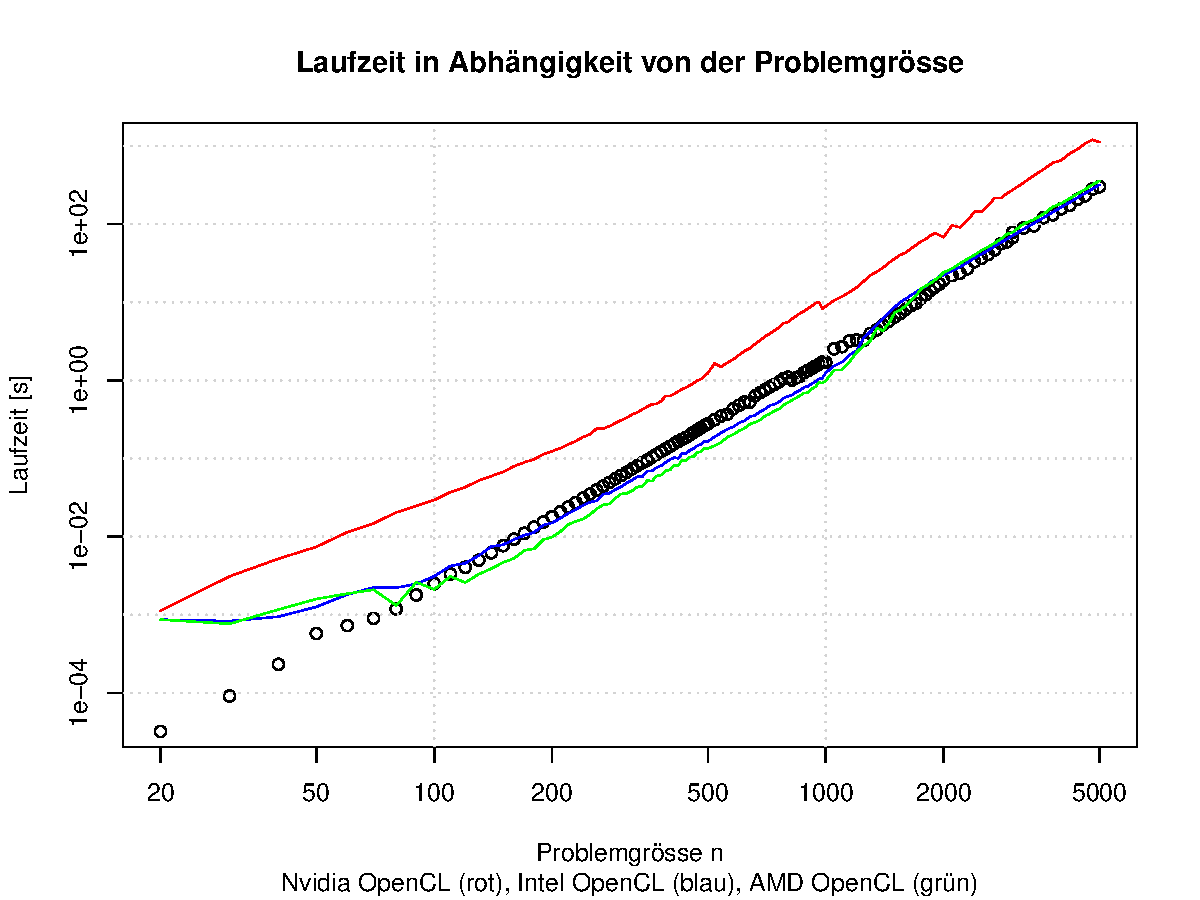
\includegraphics[width=\hsize]{images/gauss-opencl.pdf}
\end{center}
\caption{Laufzeit der OpenCL-Implementation des Gauss-Algorithmus.
Dargestellt sind
zwei CPU-basiert OpenCL Implementation von AMD (gr"un) und Intel (blau)
und die Implementation von Nvidia auf einer Tesla M2090 Karte (rot).
Zum Vergleich die unbeschleunigte C-Version in schwarz.
\label{opencl-results}}
\end{figure}

\begin{figure}
\begin{center}
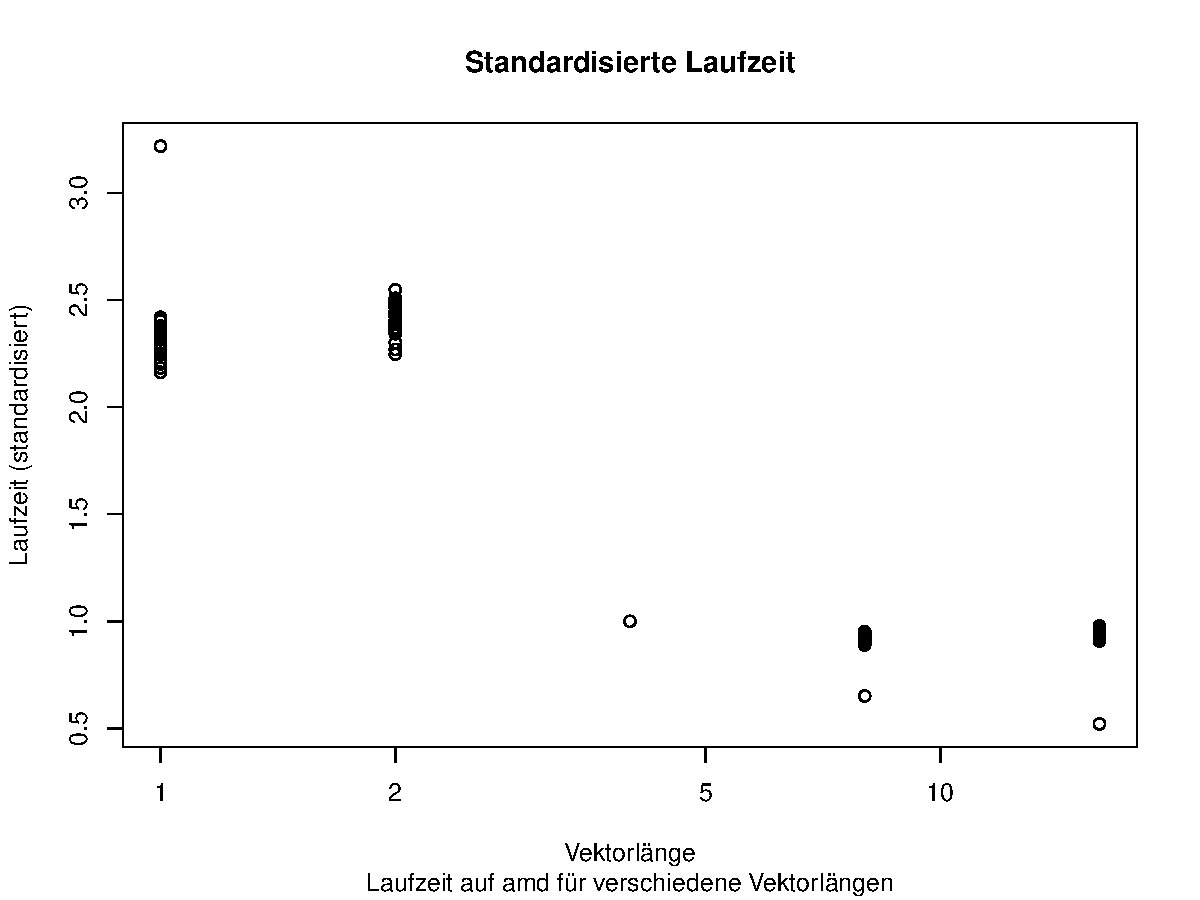
\includegraphics[width=\hsize]{images/vector-amd.pdf}
\end{center}
\caption{Laufzeit gegen Vektorgr"osse der AMD-Implementation von OpenCL.
Laufzeiten f"ur Problemgr"ossen zwischen 500 und 1000 wurden auf die
Laufzeit f"ur Vektorl"ange 4 standardisiert.
\label{opencl-simd-amd}}
\end{figure}

\begin{figure}
\begin{center}
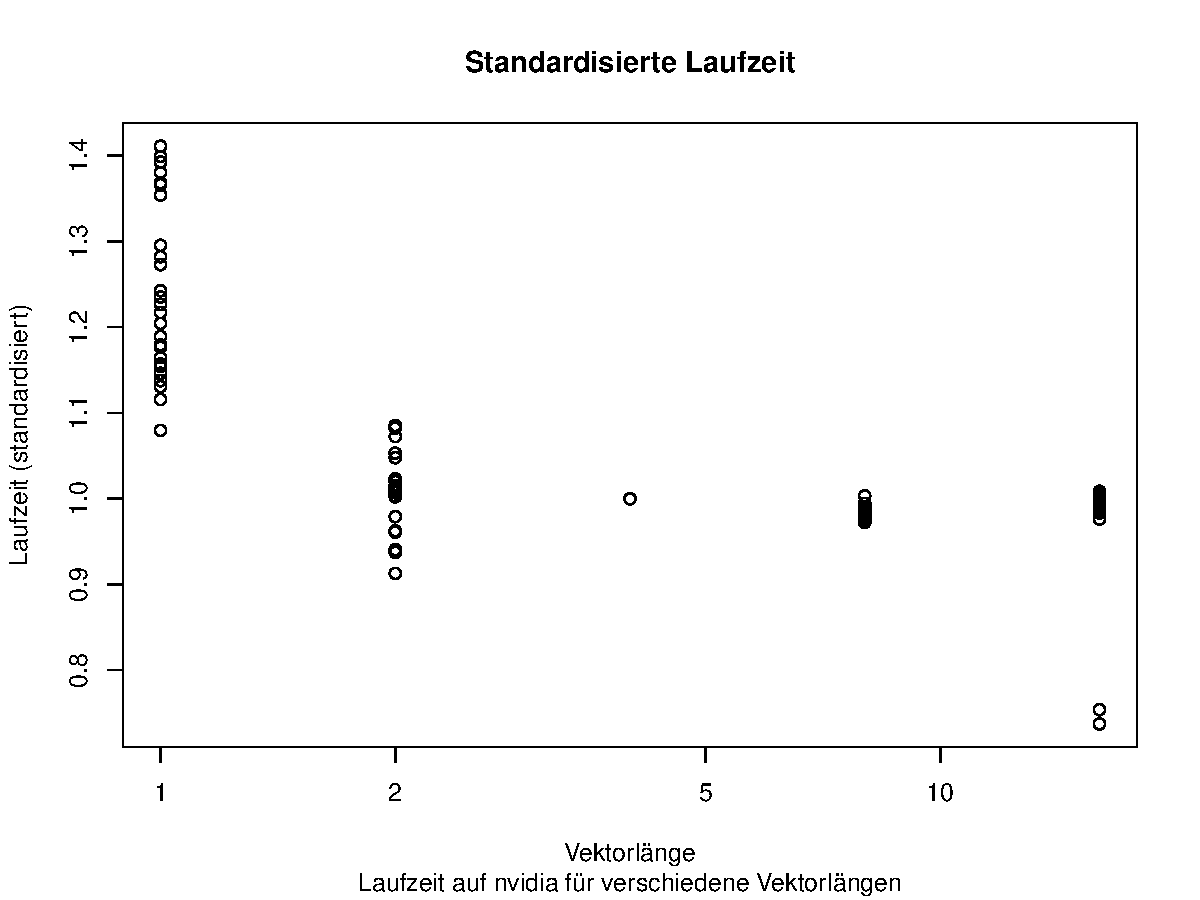
\includegraphics[width=\hsize]{images/vector-nvidia.pdf}
\end{center}
\caption{Laufzeit gegen Vektorgr"osse der Nvidia-Implementation von OpenCL.
Standardisierung wie in Abbildung \ref{opencl-simd-amd}.
\label{opencl-simd-nvidia}}
\end{figure}

\section{Message Passing: OpenMPI}
\rhead{OpenMPI}
In den Abschnitten~\ref{openmp-intro} und \ref{opencl-intro}
hat sich gezeigt, dass sich damit nur Probleme effizient l"osen lassen,
die in einem einzigen Adressraum untergebracht werden k"onnen.
Der Parallelisierung sind damit jedoch wegen des nicht gleichm"assigen
Speicherzugriffs Grenzen gesetzt.
Viele Probleme zum Beispiel aus der Str"omungsdynamik oder
der Quantenfeldtheorie sind ausserdem bedeutend gr"osser, so dass sie
auf eine grosse Zahl von Computern verteilt werden m"ussen.
Jeder Prozessor greift dadurch nur noch auf eine begrenzte Menge von Speicher
zu, er ist zudem der einzige Nutzer dieses Speichers, so dass Probleme
der Cache-Koh"arenz oder des ungleichm"assigen Zugriffs keine
Einschr"ankung mehr sind.
Es bleibt jedoch das Problem, dass einzelne Berechnungsschritte
von anderen Schritten abh"angig sind, die m"oglicherweise auf anderen
Computern berechnet wurden.
Eine solche L"osung l"asst sich also nur dann effizient realisieren,
wenn man eine Programmierungebung zur Verf"ugung hat, welche folgende
Funktionen bereitstellt:
\begin{enumerate}
\item Starten und Stoppen einer grossen Zahl von Prozessen auf vielen
Maschinen.
\item Datenaustausch zwischen den einzelnen Prozessen, abh"angig von den
Erfordernissen des Algorithmus.
Der Datenaustausch muss dabei auch ber"ucksichtigen, dass verschiedene
Prozessoren verschiedene bin"are Formate f"ur Zahlen verwenden
k"onnen, und die Daten entsprechend konvertieren. Es reicht also nicht,
einfach nur Datenbl"ocke durch TCP-Verbindungen zu schieben.
\item Konsolidierung der Daten von verschiedenen Prozessen und Output.
\end{enumerate}

H"ochste Performance kann nur dann erwartet werden, wenn die Latenz, 
die der Datenaustausch zwischen Knoten einf"uhrt, minimiert werden kann.
Spezialisierte Hardware wie Myrinet oder Infiniband kann die Latenz
eines komplexen Netzwerkstacks wie TCP/IP reduzieren, und damit
die Latenz niedrig halten, doch sollten Programm unabh"angig von solchen
Technologien geschrieben werden k"onnen.

OpenMPI l"ost genau dieses Problem.
Auf der OpenMPI Website \url{www.openmpi.org} findet man
eine grosse Menge Informationen zu OpenMPI. 
OpenMPI ist so gestaltet, dass der Entwickler ein einziges Programm
schreibt, welches dann auf einer grossen Zahl von Rechnern
ausgef"uhrt wird. Jedes Programm kann alle Resourcen eines Knotens nutzen,
es kann sogar mehrere Threads verwenden, oder ein OpenCL Compute
Device, welches auf dem Knoten verf"ugbar ist.

Jede Kopie des Programms muss also aus der Laufzeitumgebung
ableiten k"onnen, welchen Teil der Gesamtarbeit es auszuf"uhren hat.
Dazu dienen API-Funktionen, mit denen das Programm feststellen kann,
wieviele Kopien laufen und welche Nummer die aktuelle Kopie hat.
\begin{verbatim}
// initialize MPI
ierr = MPI_Init(&argc, &argv);

// get MPI dimension parameters
ierr = MPI_Comm_rank(MPI_COMM_WORLD, &rank);
ierr = MPI_Comm_size(MPI_COMM_WORLD, &num_procs);
\end{verbatim}
Die Funktion \verb+MPI_Init+ initialisiert OpenMPI, danach kann mit
den Funtionen \verb+MPI_Comm_size+ die Anzahl der Prozesse und mit
\verb+MPI_Comm_rank+ der Rang, also die Nummer, des aktuellen Prozesses
ermittelt werden.

Wie man einen parallelen Algorithmus basierend auf Rang und Anzahl
Prozesse konfigurieren kann, zeigen wir im n"achsten Abschnitt am
Beispiel das Gauss-Algorithmus.

Zum Starten der Prozesse stellt OpenMPI ein Program \verb+mpirun+
zur Verf"ugung. Zum Beispiel kann man das Beispielprogramm mit der
Implementation des Gauss-Algorithmus mit dem Befehl
\begin{verbatim}
$ mpirun -np 8 ./gauss 
\end{verbatim}
starten.

\subsection{Gauss-Algorithmus mit OpenMPI}
Die OpenMPI-Implementation des Gauss-Algorithmus richtet sich nach
den Implementationen in OpenMP und OpenCL.
Zun"achst muss die Matrix erzeugt werden, die invertiert werden soll.
Dieser Teil der Arbeit ist nicht parallelisierbar, daher wird nur Prozess 0
mit dieser Aufgabe betraut.

Die Matrix wird in Teile aufgeteilt, jeder Prozess erh"alt nur einen
Teil der Zeilen, f"ur deren Berabeitung der Prozess zust"andig ist. 
Der Bereich von Zeilenindizes, f"ur die ein Prozess verantwortlich ist,
kann aus Rang und Prozesszahl abgeleitet werden:
\begin{verbatim}
float   blocksize = n / (float)num_procs;
int     minrow = round(rank * blocksize);
int     maxrow = round((rank + 1) * blocksize);
int     height = maxrow - minrow;
\end{verbatim}
Mit Hilfe dieser Formeln kann auch jeder andere Prozess herausfinden,
wer f"ur eine bestimmte Zeile verantwortlich ist.
Der Prozess 0 sendet jetzt also den Prozessen mit Rang $r>0$ den Teil
der Matrix, f"ur den dieser zust"andig ist:
\begin{verbatim}
for (int r = 1; r < num_procs; r++) {
        int     fromrow = round(r * blocksize);
        int     torow = round((r + 1) * blocksize);
        int     h = torow - fromrow;
        memcpy(buffer, A + fromrow * n, h * n * sizeof(float));
        MPI_Send(buffer, h * n, MPI_FLOAT, r, tag, MPI_COMM_WORLD);
}
\end{verbatim}
Der Prozess mit dem Rang $r$ (viertes Argument der Funktion
\verb+MPI_Send+ empf"angt diese Daten mit Hilfe der Funktion
\verb+MPI_Recv+, und ermittelt die Anzahl der tats"achlich erhaltenen
Floats:
\begin{verbatim}
ierr = MPI_Recv(buffer, height * n, MPI_FLOAT, 0, tag,
        MPI_COMM_WORLD, &status);
int     count;
MPI_Get_count(&status, MPI_FLOAT, &count);
\end{verbatim}
Damit sind die Daten auf alle Prozesse verteilt.

In jeder Iteration des Algorithmus muss jetzt zuerst die Pivot-Zeile
durch das Pivot-Element dividiert werden. Diese Operation wird von
demjenigen Prozess durchgef"uhrt, der die Pivot-Zeile (mit Index $i$) besitzt:
\begin{verbatim}
int     sender;
for (sender = 0; sender < num_procs; sender++) {
        if ((round(sender * blocksize) <= i)
                && (i < round((sender + 1) * blocksize))) {
                break;
        }
}
\end{verbatim}
Die Schleife terminiert, sobald die aktuelle Zeile $i$ zwischen
den Grenzen liegt, f"ur die der Prozess mit der Nummer \verb+sender+
verantwortlich ist.

Der als Versender der Pivotzeile identifizierte Prozess berechnet
dann die Division durch das Pivot-Element, und kopiert die Resultate
in einen speziellen Puffer f"ur die Pivot-Zeile \verb+p+:
\begin{verbatim}
if (sender == rank) {
        // compute the pivot row
        float   pivot = a[2 * n * (i - minrow) + i];
        for (int j = 0; j < 2 * n; j++) {
                a[2 * n * (i - minrow) + j] /= pivot;
                p[j] = a[2 * n * (i - minrow) + j];
        }
}
\end{verbatim}
Der Inhalt der Pivot-Zeile muss jetzt mit allen anderen Prozessen
synchronisert werden.
Dazu rufen alle Prozesse die Funktion
\begin{verbatim}
MPI_Bcast(p, 2 * n, MPI_FLOAT, sender, MPI_COMM_WORLD);
\end{verbatim}
aus. Sie stellt sicher, dass alle Prozesse nach dem Aufruf im Puffer \verb+p+
die Daten haben, welche der Prozess \verb+sender+ berechnet hat.

Erst wenn die Daten synchronisiert sind k"onnen die einzelnen Prozesse
weiterlaufen, es ist also kein spezielles Barrier-Konstrukt n"otig.
Der Code f"ur die Zeilenoperationen unterscheidet sich nicht von den
anderen Implementationen.

Wenn die Berechnung abgeschlossen ist, m"ussen die berechneten Teile
der invertierten Matrix wieder von Prozess 0 gesammelt werden.

\subsection{Resultate}
\begin{figure}
\begin{center}
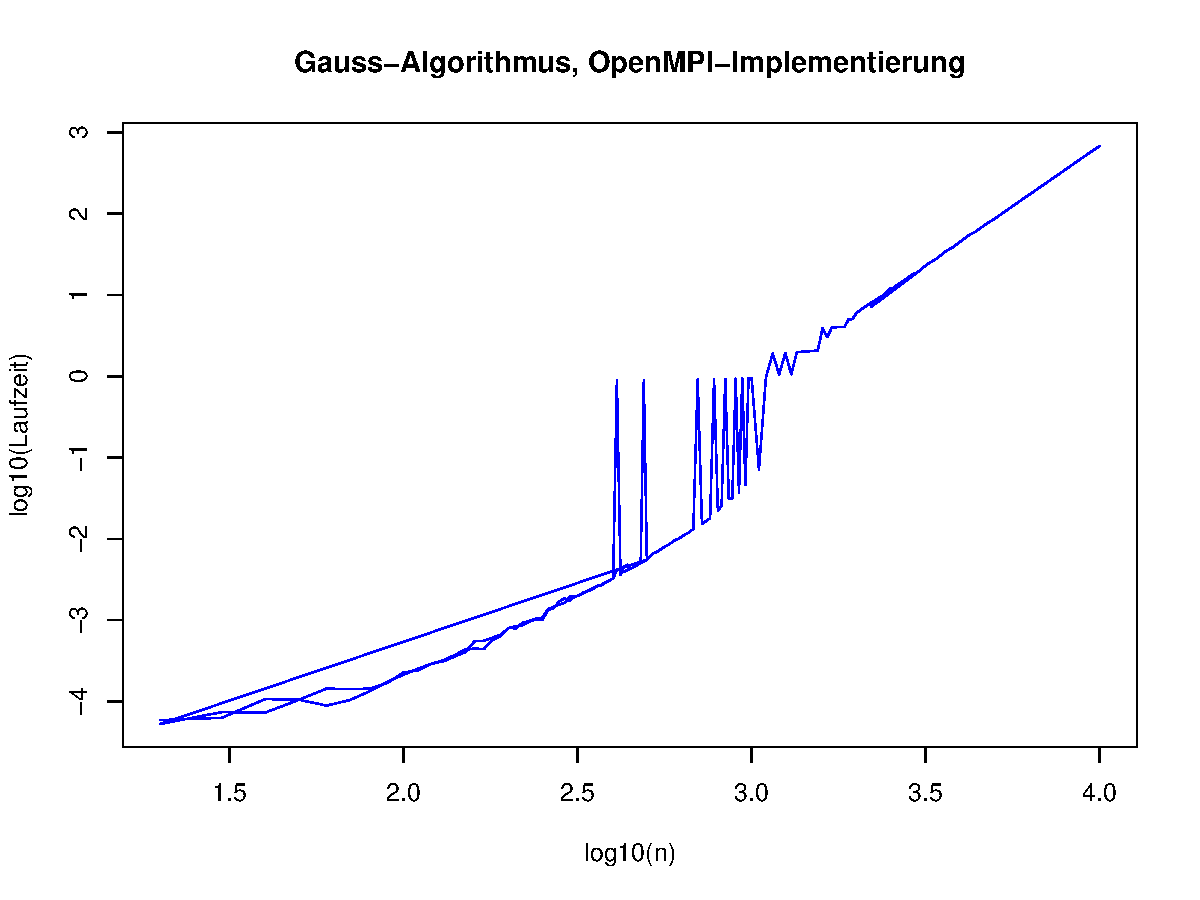
\includegraphics[width=\hsize]{images/gauss-openmpi.pdf}
\end{center}
\caption{Laufzeit der OpenMPI-Implementierung des Gauss-Algorithmus.
Die blaue Kurve zeigt die Laufzeit mit 32 Prozessen, rot sind die
Vergleichsmessung der sequenziellen Implementation eingetragen.
\label{openmpi-performance}}
\end{figure}
Die Laufzeitmessungen in Abbildung \ref{openmpi-performance} zeigen,
dass die OpenMPI-Implementation schon bei kleinen Problemen schneller
l"auft als die OpenMP-Implementation.
Bei kleienn Problemn unter $n=100$ ist der OpenMPI Overhead dominant.
Gegen"uber der Pthread-Implementation zeigt sich auch ein deutlich gr"osserer
Performance-Gewinn durch Verwendung mehrerer Threads.
Es ist allerdings auch schon erkennbar, dass die grosse Zahl von 32 Threads
kaum mehr zus"atzliche Performance bringt.

\begin{figure}
\begin{center}
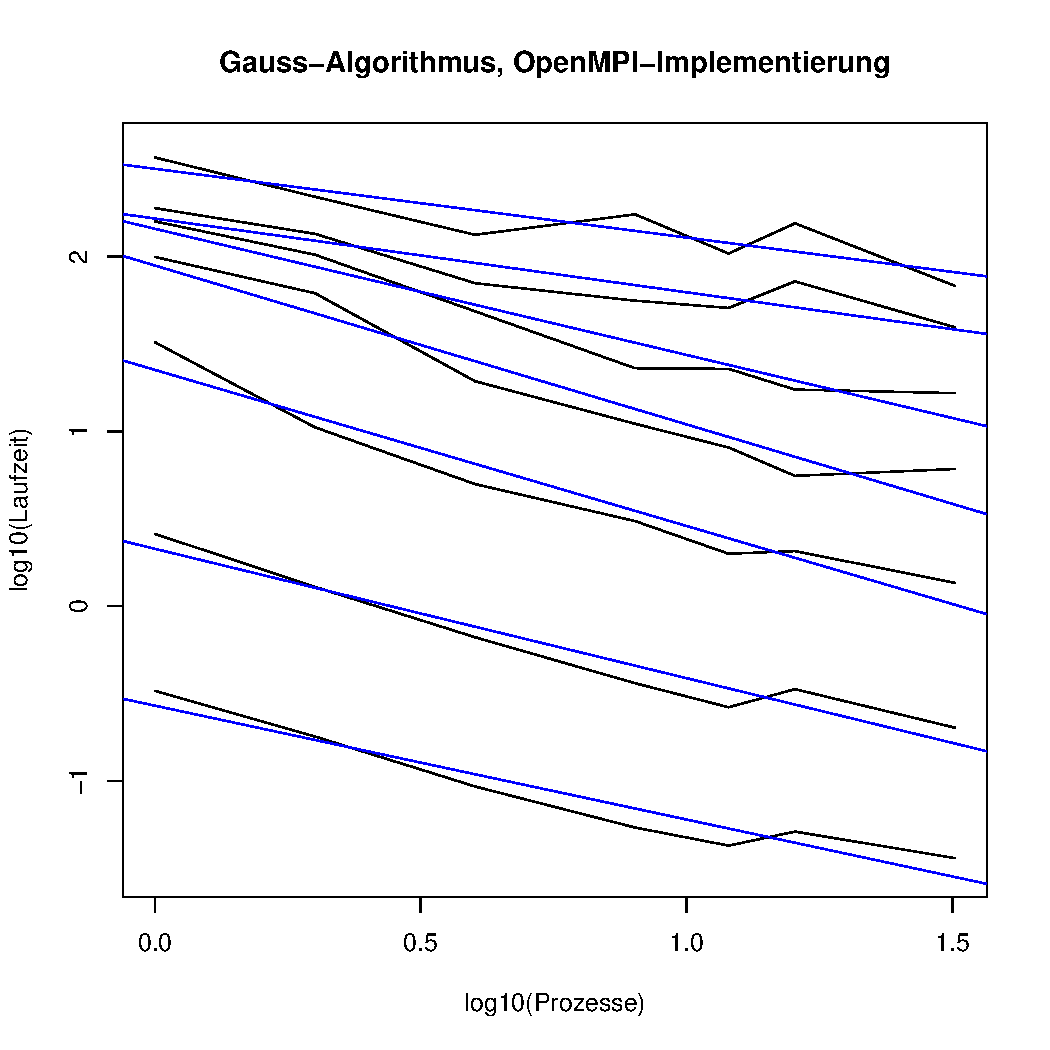
\includegraphics[width=\hsize]{images/gauss-threads.pdf}
\end{center}
\caption{Laufzeit in Abh"angigkeit von der Anzahl Prozesse.
F"ur weninger als 16 Prozesse skaliert der Algorithmus sehr viel besser.
F"ur $n>3500$ (drittoberste Kurve) ist erkennbar, wie die Skalierung
zusammenbricht. 
Von oben nach unten ist $n=5000$, $4000$, $3500$, $3000$, $2000$, $1000$
und $500$.
\label{openmpi-threads}}
\end{figure}
In Abbildung \ref{openmpi-threads} ist die Abh"angigkeit der Laufzeit von
der Anzahl der Prozesse von dargestellt. Mehr als 12 Threads bringen
keinen Laufzeitverbesserung mehr. Ebenso skaliert die L"osung f"ur 
Problem nicht mehr, wenn $n$ wesentlich gr"osser als ca.~3000 ist.

\section{Gegen"uberstellung}
Diese Fallbeispiele und insbesondere auch die Performance-Auswertungen
geben einen ziemlich guten "Uberblick "uber die angemessenen Anwendungsgebiete
der einzelnen Technologien.

Parallelisierung mit Pthreads ist nur in den seltensten F"allen sinnvoll.
Der Programmieraufwand ist zu gross, die so erzeugten Threads m"ussen
m"uhsam ``von Hand'' synchronisiert werden, und da sie ansonsten
vollst"andig entkoppelt, hat man keine Kontrolle "uber den Schaden,
den sie m"oglicherweise durch ung"unstige Zugriffsmuster im Cache anrichten.

OpenMP ist die richtige Parallelisierungstechnik f"ur Aufgaben, die
wegen zu starker Kopplung der verschiedenen Berechnungsteile untereinander
in einem einzigen Prozess abgewickelt werden m"ussen.
Besondere Vorsicht ist dabei darauf zu verwenden, dass die Zahl der
Threads richtig gew"ahlt wird, und dass richtige Semantik f"ur
lokale Variablen umgesetzt wird.

OpenCL bietet sich f"ur Anwendungen an, die sich auf das etwas spezielle
Ausf"uhrungsmodell anpassen lassen. Dabei ist wichtig, dass die
Work-Items m"oglichst unabh"angig sind, da sonst die Anzahl der Work-Groups
reduziert wird, und Synchronisation innerhalb einer Workgroup mit
sehr schlechter Performance einhergeht.

Grosse Problem m"ussen mit OpenMPI angepackt werden. Nur so kann man
auf eine Vielzahl von Maschinen skalieren. Innerhalb der einzelnen
Prozesse k"onnen selbstverst"andlich Techniken wie OpenMP oder OpenCL 
zum Einsatz kommen.
Bei kleinen Problemen ist der Startup-Overhead von OpenMPI problematisch,
doch schon Probleme moderater Gr"osse k"onnen in einer OpenMPI Implementation
auf einer einzelnen Maschine effizienter sein als OpenMP, weil die
einzelnen Prozesse getrennten Speicher verwenden. Als Folge m"ussen die
Algorithmen so gestaltet sein, dass keine zwei Threads den gleichen
Speicher brauchen, damit ist es auch nicht m"oglich, dass verschiedene
Threads sich gegenseitig den Cache f"ur das gleiche Problem streitig machen.


